We tested our language by various examples.

\subsection{The Dice Program}
 The first example we present is the Dice Program\footnote{\url{https://www.prismmodelchecker.org/casestudies/dice.php}} \cite{KY76}. The following program models a die using only fair coins. Starting at the root vertex (state 0), one repeatedly tosses a coin. Every time heads appears, one takes the upper branch and when tails appears, the lower branch. This continues until the value of the die is decided.


\begin{figure}[h]
\centering

\includegraphics[scale=0.6]{diagram-20230725.pdf}	
\end{figure}

We modelled the program using the choreographic language (Listing \ref{ex1-code}) and we were able to generate the corresponding PRISM program, reported in Listing \ref{ex1-gen}.

\begin{lstlisting}[style=chor-color,caption={Choreographic language for the Dice Program.},captionpos=b,label={ex1-code}]
preamble
"dtmc"
endpreamble

n = 1;
Dice $\rightarrow$ Dice : "d : [0..6] init 0;" ;

{
DiceProtocol$_0$ $\coloneqq$ Dice $\rightarrow$ Dice : (+["0.5*1"]  " "$\&\&$" " . DiceProtocol$_1$
                                    +["0.5*1"]  " "$\&\&$" " .  DiceProtocol$_2$)

DiceProtocol$_1$ $\coloneqq$ Dice $\rightarrow$ Dice : (+["0.5*1"]  " "$\&\&$" " . 
 			Dice $\rightarrow$ Dice : (+["0.5*1"]  " "$\&\&$" " . DiceProtocol$_1$
           	 		 	+["0.5*1"]  "(d'=1)"$\&\&$" " . DiceProtocol$_3$)
     				   +["0.5*1"]  " "$\&\&$" " .  
   			Dice $\rightarrow$ Dice : (+["0.5*1"]  "(d'=2)"$\&\&$" " . DiceProtocol$_3$
           	 		         +["0.5*1"]  "(d'=3)"$\&\&$" " . DiceProtocol$_3$))

DiceProtocol$_2$ $\coloneqq$ Dice $\rightarrow$ Dice : (+["0.5*1"]  " "&&" " . 
	 		Dice $\rightarrow$ Dice : (+["0.5*1"]  " "&&" " . DiceProtocol$_2$
	 	                	 +["0.5*1"]  "(d'=4)"$\&\&$" " . DiceProtocol$_3$)
	 			 +["0.5*1"]  " "&&" " . 
	    		Dice $\rightarrow$ Dice : (+["0.5*1"]  "(d'=5)"$\&\&$" " . DiceProtocol$_3$
	                     		+["0.5*1"]  "(d'=6)"$\&\&$" " . DiceProtocol$_3$))

DiceProtocol$_3$ $\coloneqq$ Dice $\rightarrow$ Dice : (["1*1"] " "$\&\&$" ".DiceProtocol$_3$)
}
	
\end{lstlisting}


\begin{lstlisting}[style=prism-color,caption={Generated PRISM program for the Dice Program.},captionpos=b,label={ex1-gen}]
dtmc

module Dice
	Dice : [0..11] init 0;
	d : [0..6] init 0; 

	[] (Dice=0)  $\rightarrow$ 0.5 :  (Dice'=2) + 0.5 :  (Dice'=6); 
	[] (Dice=2)  $\rightarrow$ 0.5 :  (Dice'=3) + 0.5 :  (Dice'=4); 
	[] (Dice=3)  $\rightarrow$ 0.5 :  (Dice'=2) + 0.5 : (d'=1)&(Dice'=10); 
	[] (Dice=4)  $\rightarrow$ 0.5 : (d'=2)$\&$(Dice'=10) + 0.5 : (d'=3)$\&$(Dice'=10);
	[] (Dice=6)  $\rightarrow$ 0.5 :  (Dice'=7) + 0.5 : (Dice'=8); 
	[] (Dice=7)  $\rightarrow$ 0.5 :  (Dice'=6) + 0.5 : (d'=4)$\&$(Dice'=10);
	[] (Dice=8)  $\rightarrow$ 0.5 : (d'=5)$\&$(Dice'=10) + 0.5 : (d'=6)$\&$(Dice'=10); 
	[] (Dice=10)  $\rightarrow$ 1 :  (Dice'=10);

endmodule
	
\end{lstlisting}

By comparing our model with the one presented in the PRISM documentation, we noticed that the difference is the number assumed by the variable {\tt Dice}. In particular, the variable does not assume the values 1, 5 and 9. This is due to how the generation in presence of a branch is done. However, this does not cause any problems since the updates are done correctly.
Moreover,  to prove the generated program is correct, we show that the probability of reaching a state where 
$$\texttt{d=k} \text{ for } \texttt{k}=1,\ldots,6 \text{ is } 1/6.$$
The results are displayed in Figure \ref{ex1-res}, where also the results obtained with the original PRISM model are shown.
\begin{figure}[h]
\centering
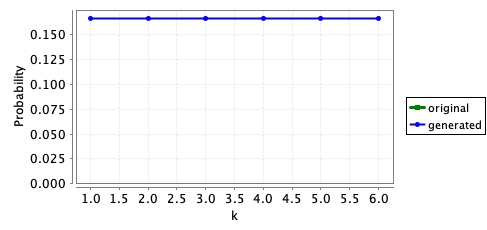
\includegraphics[scale=0.6]{example2-results.jpeg}	
\caption{Probability of reaching a state where $d=k$, for $k=1,\ldots,6.$}
\label{ex1-res}
\end{figure}

\subsection{Simple Peer-To-Peer Protocol}
This case study describes a simple peer-to-peer protocol based on BitTorrent\footnote{\url{https://www.prismmodelchecker.org/casestudies/peer2peer.php}}. The model comprises a set of clients trying to download a file that has been partitioned into $K$ blocks. Initially, there is one client that has already obtained all of the blocks and $N$ additional clients with no blocks. Each client can download a block from any of the others but they can only attempt four concurrent downloads for each block.\\
The code we analyze with $k=5$ and $N=4$ is reported in Listing \ref{ex2-code}.
\begin{lstlisting}[style=chor-color,caption={Choreographic language for the Peer-To-Peer Protocol.},captionpos=b,label={ex2-code}]
preamble
"ctmc"
"const double mu=2;"
"formula rate1=mu*(1+min(3,b11+b21+b31+b41));"
"formula rate2=mu*(1+min(3,b12+b22+b32+b42));"
"formula rate3=mu*(1+min(3,b13+b23+b33+b43));"
"formula rate4=mu*(1+min(3,b14+b24+b34+b44));"
"formula rate5=mu*(1+min(3,b15+b25+b35+b45));"
endpreamble

n = 4;
n = 4;

Client[i] $\rightarrow$ i in [1...n]
Client[i] : "b[i]1 : [0..1];", "b[i]2 : [0..1];", "b[i]3 : [0..1];", "b[i]4 : [0..1];", "b[i]5 : [0..1];" ;

{
PeerToPeer := Client[i] $\rightarrow$ Client[i]: 
			(+["rate1*1"]  "(b[i]1'=1)"$\&\&$" " . PeerToPeer
			 +["rate2*1"]  "(b[i]2'=1)"$\&\&$" " . PeerToPeer
			 +["rate3*1"]  "(b[i]3'=1)"$\&\&$" " . PeerToPeer
			 +["rate4*1"]  "(b[i]4'=1)"$\&\&$" " . PeerToPeer
			 +["rate5*1"]  "(b[i]5'=1)"$\&\&$" " . PeerToPeer)
}
	
\end{lstlisting}

Part of the generated PRISM code is shown in Listing \ref{ex2-gen} and it is faithful with what reported in the PRISM documentation. 
\begin{lstlisting}[style=prism-color,caption={Generated PRISM program for the Peer-To-Peer Protocol.},captionpos=b,label={ex2-gen}]
ctmc
const double mu=2;
formula rate1=mu*(1+min(3,b11+b21+b31+b41));
formula rate2=mu*(1+min(3,b12+b22+b32+b42));
formula rate3=mu*(1+min(3,b13+b23+b33+b43));
formula rate4=mu*(1+min(3,b14+b24+b34+b44));
formula rate5=mu*(1+min(3,b15+b25+b35+b45));

module Client1
	Client1 : [0..1] init 0;
	b11 : [0..1]; 
	b12 : [0..1]; 
	b13 : [0..1]; 
	b14 : [0..1]; 
	b15 : [0..1]; 

	[] (Client1=0)  $\rightarrow$ rate1 : (b11'=1)$\&$(Client1'=0); 
	[] (Client1=0)  $\rightarrow$ rate2 : (b12'=1)$\&$(Client1'=0); 
	[] (Client1=0)  $\rightarrow$ rate3 : (b13'=1)$\&$(Client1'=0); 
	[] (Client1=0)  $\rightarrow$ rate4 : (b14'=1)$\&$(Client1'=0); 
	[] (Client1=0)  $\rightarrow$ rate5 : (b15'=1)$\&$(Client1'=0); 
	
endmodule
	
\end{lstlisting}


In Figure \ref{ex2-res}, we compare the values obtained for the probability that all clients have received all blocks by time $0\leq T\leq 1.5$ both for our generated model and the model reported in the documentation.
\begin{figure}[h]
\centering
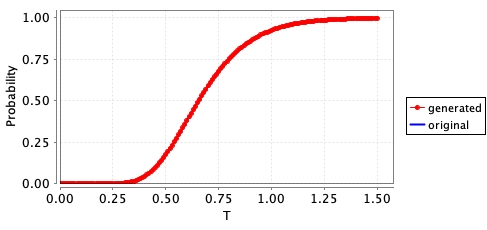
\includegraphics[scale=0.6]{example3-results.jpeg}	
\caption{Probability that clients received all the block before $T$, with $0\leq T \leq 1.5$.}
\label{ex2-res}
\end{figure}

\subsection{Proof of Work Bitcoin Protocol}
This protocol represents the Proof of Work implemented in the Bitcoin blockchain.
In\cite{DBLP:journals/concurrency/BistarelliNGLMV23}, a Bitcoin system is the result of the parallel composition of $n$ Miner processes, $n$  \emph{Hasher} processes and a process called \emph{Network}.
\emph{Hasher} processes model the attempts of the miners to solve the cryptopuzzle, while the \emph{Network} process model the broadcast communication among miners. 
We tested our system by considering a protocol with $n=5$ miners and it is reported in Listing \ref{ex3-code}.
\begin{lstlisting}[style=chor-color,caption={Choreographic language for the Proof of Work Bitcoin Protocol.},captionpos=b,label={ex3-code}]
preamble
"ctmc"
"const T"
"const double r = 1;"
"const double mR = 1/600;"
"const double lR = 1-mR;"
"const double hR1 = 0.25;"
"const double hR2 = 0.25;"
"const double hR3 = 0.25;"
"const double hR4 = 0.25;"
"const double rB = 1/12.6;"
"const int N = 100;"
endpreamble

n = 4;

Hasher[i] -> i in [1...n] ;

Miner[i] -> i in [1...n]
Miner[i] : "b[i] : block {m[i],0;genesis,0} ;", "B[i] : blockchain [{genesis,0;genesis,0}];" ,"c[i] : [0..N] init 0;", "setMiner[i] : list [];" ;

Network ->
Network : "set1 : list [];", "set2 : list [];", "set3 : list [];" , "set4 : list [];"; 
	
{
PoW := Hasher[i]  $\rightarrow$  Miner[i] :
(+["mR*hR[i]"]  " "$\&\&$"(b[i]'=createB(b[i],B[i],c[i]))&(c[i]'=c[i]+1)" . 
	Miner[i]  $\rightarrow$  Network : 
		(["rB*1"] "(B[i]'=addBlock(B[i],b[i]))" $\&\&$ 
		foreach(k != i) "(set[k]'=addBlockSet(set[k],b[i]))" @Network .PoW)
 +["lR*hR[i]"] " " $\&\&$ " " .
 	if "!isEmpty(set[i])"@Miner[i] then { 
  		["r"] "(b[i]'=extractBlock(set[i]))"@Miner[i] . 
			Miner[i]  $\rightarrow$  Network : 
			(["1*1"] "(setMiner[i]' = addBlockSet(setMiner[i] , b[i]))"$\&\&$"(set[i]' = removeBlock(set[i],b[i]))" . PoW) 
 	}
 	else{
 		if "canBeInserted(B[i],b[i])"@Miner[i] then { 
 			["1"] "(B[i]'=addBlock(B[i],b[i]))
			&(setMiner[i]'=removeBlock(setMiner[i],b[i]))"@Miner[i] . Pow 
 		}
 		else{
 			PoW
		}
	}
)
} 	
\end{lstlisting}

Part of the generated PRISM code is shown in Listing \ref{ex3-gen}. 
\begin{lstlisting}[style=prism-color,caption={Generated PRISM program for the Peer-To-Peer Protocol.},captionpos=b,label={ex3-gen}]
ctmc
const T;
const double r = 1;
const double mR = 1/600;
const double lR = 1-mR;
const double hR1 = 0.25;
const double hR2 = 0.25;
const double hR3 = 0.25;
const double hR4 = 0.25;
const double rB = 1/12.6;
const int N = 100;

module Miner1
Miner1 : [0..7] init 0;
b1 : block {m1,0;genesis,0} ; 
B1 : blockchain [{genesis,0;genesis,0}]; 
c1 : [0..N] init 0; 
setMiner1 : list []; 

[PZKYT] (Miner1=0)   $\rightarrow$  hR1 : (b1'=createB(b1,B1,c1))$\&$(c1'=c1+1)$\&$(Miner1'=1); 
[EUBVP] (Miner1=0)   $\rightarrow$  hR1 :  (Miner1'=2); 
[HXYKO] (Miner1=1)   $\rightarrow$  1 : (B1'=addBlock(B1,b1))$\&$(Miner1'=0); 
[] (Miner1=2)$\&$!isEmpty(set1)  $\rightarrow$  r : (b1'=extractBlock(set1))$\&$(Miner1'=4); 
[SRKSV] (Miner1=4)   $\rightarrow$  1 : (setMiner1' = addBlockSet(setMiner1 , b1))$\&$(Miner1'=0); 
[] (Miner1=2)$\&$!(!isEmpty(set1))  $\rightarrow$  1 : (Miner1'=5); 
[] (Miner1=5)$\&$canBeInserted(B1,b1)  $\rightarrow$  1 : (B1'=addBlock(B1,b1))
		$\&$(setMiner1'=removeBlock(setMiner1,b1))$\&$(Miner1'=0); 
[] (Miner1=5)$\&$!(canBeInserted(B1,b1))  $\rightarrow$  1 : (Miner1'=0);
endmodule
$\ldots$
module Network
Network : [0..1] init 0;
set1 : list []; 
$\ldots$

[HXYKO] (Network=0)  $\rightarrow$  1 : (set2'=addBlockSet(set2,b2))$\&$(set3'=addBlockSet(set3,b3))$\&$(set4'=addBlockSet(set4,b4))$\&$(Network'=0); 
[SRKSV] (Network=0)  $\rightarrow$  1 : (set1' = removeBlock(set1,b1))$\&$(Network'=0); 
$\ldots$

endmodule

module Hasher1
Hasher1 : [0..1] init 0;

[PZKYT] (Hasher1=0)  $\rightarrow$  mR :  (Hasher1'=0); 
[EUBVP] (Hasher1=0)  $\rightarrow$  lR :  (Hasher1'=0); 

endmodule
\end{lstlisting}


In Figure \ref{ex2-res}, we compare the values obtained for the probability that at least one miner has mined a block both for the generated model and the model presented in \cite{DBLP:journals/concurrency/BistarelliNGLMV23}.
\begin{figure}[h]
\centering
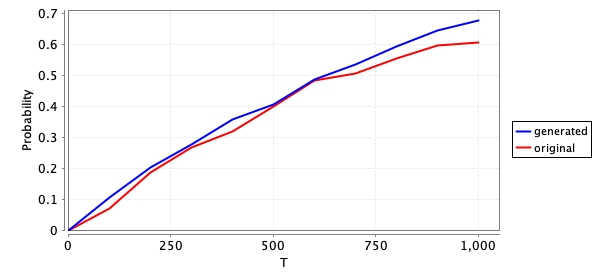
\includegraphics[scale=0.6]{example4-results.jpeg}	
\caption{Probability at least one miner has created a block.}
\label{ex3-res}
\end{figure}
%%% Local Variables: 
%%% mode: latex
%%% TeX-master: "main"
%%% End: